

%---------------------------------------------------------------------------------------------------
% Voreinstellungen (Layout, neue Befehle, etc.)
%---------------------------------------------------------------------------------------------------

%---------------------------------------------------------------------------------------------------
% Einstellungen
% (gelten nur in Zusammenarbeit mit pdflatex)
%---------------------------------------------------------------------------------------------------
\documentclass[
  pagesize,	                                           % flexible Auswahl des Papierformats
  a4paper,  	                                         % DIN A4
  oneside,    	                                       % einseitiger Druck
  BCOR5mm,      	                                     % Bindungskorrektur
  headsepline,                                         % Strich unter der Kopfzeile
  12pt,                                                % 12pt Schriftgr��e
	halfparskip,                                         % Europ�ischer Satz: Abstand zwischen Abs�tzen
	abstracton,																					 % Spezielle Formatierung, die erlaubt, dass die
																											 % Zusammenfassung vor dem Inhaltsverzeichnis steht
	%draft,																							 % Es handelt sich um eine Vorabversion	
	final,																							 % Es handelt sich um die endg�ltige Version
	liststotoc,																					 % Tabellen- und Abbildungsverzeichnis im 																																 % Inhaltsverzeichnis
	idxtotoc,																						 % Index im Inhaltsverzeichnis	
  bibtotoc,                                            % Literaturverzeichnis im Inhaltsverzeichnis  
]{scrreprt}                                            % KOMA-Scriptklasse Report

%---------------------------------------------------------------------------------------------------
\usepackage[english,ngerman]{babel}                    % deutsche Trennmuster %KAY ngerman keinen einfluss auf ziel
\usepackage{varwidth}                          % KAY !!
\usepackage{wrapfig}                           % KAY !!
\usepackage{color}                             % KAY !!
\usepackage[T1]{fontenc}                               % EC-Schriften, Trennstellen nach Umlauten
\usepackage[latin1]{inputenc}                          % direkte Umlauteingabe (� statt "a)
                                                       % latin1/latin9 f�r unixoide Systeme
                                                       % (latin1 ist auch unter Win verwendbar)
                                                       % ansinew f�r Windows
                                                       % applemac Macs
                                                       % cp850 OS/2
\usepackage{times}              											 % Schriften Paket
\usepackage{array,ragged2e} 													 % Wichtig f�r Abstandsformatierung

%---------------------------------------------------------------------------------------------------
\usepackage{cmbright}                                  % serifenlose Schrift als Standard
                                                       % + alle f�r TeX ben�tigten mathematischen
                                                       % Schriften einschlie�lich der AMS-Symbole
\usepackage[scaled=.90]{helvet}                        % skalierte Helvetica als \sfdefault
\usepackage{courier}                                   % Courier als \ttdefault

%---------------------------------------------------------------------------------------------------
\usepackage[automark]{scrpage2}                        % Anpassung der Kopf- und Fu�zeilen
\usepackage{xspace}                                    % Korrekter Leerraum nach Befehlsdefinitionen
\usepackage{setspace}																	 % Dieses Package brauchen wir f�r den 				
\usepackage[pdftex]{graphicx}
\usepackage[absolute,overlay]{textpos}         
\usepackage[final]{pdfpages}													 % anderthalbzeiligen Abstand.
\usepackage[numbers]{natbib}                                    % Neuimplementierung des \cite-Kommandos
\usepackage{bibgerm}       											       % Deutsche Bezeichnungen
\usepackage[absolute]{textpos}                         % placing boxes at absolute positions
\usepackage[final]{pdfpages}                           % include pages of external PDF documents
\usepackage{tabularx}                                  % Spaltenbreite bis zur Seitenbreite dehnen
\usepackage{makeidx}																	 % Paket zur Erstellung eines Stichwortverzeichnisses
\makeindex																						 % Automatische Erstellung des Stichwortverzeichnis
\usepackage[intoc,
						english,
						prefix]{nomencl}
\makenomenclature

%---------- Selbst hinzugef�gt (Krystian Bolz)
%\newcommand*{\SVG}{}																	% Comment out if SVG package is not correct available
\newcommand{\figwidthoctave}{12.5cm}														% Figure Width for Octave Plots
\newcommand{\figwidthgnuplot}{10cm}														% Figure Width for Gnuplot Plots

\usepackage{acronym}																	% Acronym Umgebung f�r Abk�rzungen
\usepackage{amsmath}																	% Mathe Umgebung
\numberwithin{equation}{chapter}											% Nummerierung der Formeln nach Kapiteln
\usepackage{float}
\usepackage{amssymb}% http://ctan.org/pkg/amssymb
\usepackage{pifont}% http://ctan.org/pkg/pifont
\usepackage{subfigure} % Mehrere Bilder nebeneinander
\usepackage{forloop} % F�r Schleife im Anhang
\usepackage{listings} % Quellcode
\usepackage{color} % Syntax Highlighting Quellcode

\addto\captionsngerman{\renewcommand{\bibname}{Quellenverzeichnis}} % Neue Literaturverzeichnis �berschrift

\definecolor{gray}{rgb}{0.4,0.4,0.4}
\definecolor{darkblue}{rgb}{0.0,0.0,0.6}
\definecolor{cyan}{rgb}{0.0,0.6,0.6}

\lstset{
  basicstyle=\small,
  columns=fullflexible,
  showstringspaces=false,
  commentstyle=\color{gray}\upshape
}

\lstdefinelanguage{XML}
{
  morestring=[b]",
  morestring=[s]{>}{<},
  morecomment=[s]{<?}{?>},
  stringstyle=\color{black},
  identifierstyle=\color{darkblue},
  keywordstyle=\color{cyan},
  morekeywords={xmlns,version,type}% list your attributes here
}

\ifdefined\SVG
\usepackage{svg}																			% F�r Vektorgrafiken
\fi

%---------------------------------------------------------------------------------------------------
 \usepackage{graphicx}                                 % Zur Einbindung von PDF-Bildern
 \usepackage[colorlinks,															 % Einstellen und Laden des Hyperref-Pakets
	pdftex,
	bookmarks,
	bookmarksopen=false,
	bookmarksnumbered,
	citecolor=black, % was blue
	linkcolor=black, % was blue
	urlcolor=black, % was blue
	filecolor=black, % was blue
	linktocpage,
  pdfstartview=Fit,                                    % startet mit Ganzseitenanzeige    
	pdfsubject={Multiagentensystemgest�tzte Clusteranalyse},
	pdftitle={Bachelorthesis im Fachbereich Elektrotechnik \& Informatik an der HAW-Hamburg},
	pdfauthor={Bj�rn Jensen, http://www.mirou.de}]{hyperref}
 \pdfcompresslevel=9
 
%---------------------------------------------------------------------------------------------------
% Inhaltsverzeichnis und Abschnittnummerierung
%---------------------------------------------------------------------------------------------------
\setcounter{secnumdepth}{2}   % Ich habe recht kurze Kapitel. Die sollen nicht durchnummeriert sein.
\setcounter{tocdepth}{2}

%---------------------------------------------------------------------------------------------------
% Abbildungsverzeichnis
%---------------------------------------------------------------------------------------------------
\graphicspath{{grafiken/}}

%---------------------------------------------------------------------------------------------------
% Kopf- und Fu�zeilen
%---------------------------------------------------------------------------------------------------
\pagestyle{scrheadings}
\clearscrheadings
\clearscrplain
\clearscrheadfoot
\ohead{\pagemark}
\ihead{\headmark}

%---------------------------------------------------------------------------------------------------
% Neue Befehle
%---------------------------------------------------------------------------------------------------
%---------------------------------------------------------------------------------------------------
% Neue Befehle
%---------------------------------------------------------------------------------------------------

%---------------------------------------------------------------------------------------------------
% Umbenennen des Symbolverzeichnisses
%---------------------------------------------------------------------------------------------------
\renewcommand{\nomname}{Glossar}				% Das Symbolverzeichnis heisst nun "Glossar"
\renewcommand{\nomlabel}[1]{						% Die zu erkl�renden Begriffe sind nun fett hervorgehoben
	\hfil \textbf{#1} \hfil
}

%---------------------------------------------------------------------------------------------------
% Ein paar ganz n�tzliche Befehle von Lars M�hlmann
%---------------------------------------------------------------------------------------------------
%f�r Kommentare 
\newcommand{\colb}{\color{green}}
\newcommand{\colbl}{\color{black}}

%---------------------------------------------------------------------------------------------------
% Befehle zum Erstellen des Index
% \addIndexEntry{Eintrag in den Index}
% \addSubIndexEntry{Eintrag in den Index}{Eintrag des �bergeordneten Eintrags}
%---------------------------------------------------------------------------------------------------
\newcommand{\addIndexEntry}[1]{#1\index{#1}}
\newcommand{\addSubIndexEntry}[2]{#1\index{#2!#1}}

%---------------------------------------------------------------------------------------------------
% LaTeX in eigenem Font
%---------------------------------------------------------------------------------------------------
\newcommand{\myLatex}{
	{\rmfamily\LaTeX\xspace}
}

%---------------------------------------------------------------------------------------------------
% Befehl zum Erstellen und Hervorheben eines Zitats
% Parameter:
% 1. Zitat
% 2. Author
% 3. Quelle
%---------------------------------------------------------------------------------------------------
\newcommand{\myCitation}[3]{
	\begin{flushright}
	\begin{minipage}{.4\linewidth}
		\footnotesize\rmfamily\itshape 
		#1 \\
		\RaggedLeft #2 \\
		#3
	\end{minipage}
	\end{flushright}
	\nobreakspace
}

%---------------------------------------------------------------------------------------------------
% Erstellung von Deckblatt (Seite 1) und Titelblatt (Seite 2)
%---------------------------------------------------------------------------------------------------
\newcommand{\createCoverAndTitlePage}[7]{
	\createCover{#1}{#2}{#3}{#4}
	\createTitlePage{#1}{#2}{#3}{#4}{#5}{#6}{#7}
}

%---------------------------------------------------------------------------------------------------
% Erstellung von Deckblatt (Seite 1) 
% Anwendung:
% \createCover{Art der Arbeit}{Typ der Arbeit}{Autor}{Titel}
%---------------------------------------------------------------------------------------------------
\newcommand{\createCover}[4]{
	\thispagestyle{empty}
	\begin{titlepage}

	\setlength{\TPHorizModule}{1mm}
	\setlength{\TPVertModule}{1mm}
	\textblockorigin{0mm}{0mm} % start everything near the top-left corner

	% Art der Arbeit
	\begin{textblock}{111}(83,115)
		\begin{minipage}[c][1,78cm][c]{11,09cm}		
  		\fontsize{22pt}{20pt}
  		\selectfont
  		\begin{center}
  		#1#2
  		\end{center}
		\end{minipage}
	\end{textblock}

	% Name & Titel
	\begin{textblock}{111}(83,131)
		\begin{minipage}[c][4,81cm][t]{11,09cm}	
		\linespread{1.2}	
    		\fontsize{16pt}{14pt}    
    		\selectfont
    		\begin{center}
    			#3 \\ \medskip    
    			#4
    		\end{center}
    		\end{minipage}
	\end{textblock}
	\begin{textblock}{111}(35,260)
		\begin{minipage}[c][1,5cm][t]{7,0cm}		
  		\fontsize{10pt}{10pt}
  		\selectfont
		\textit{
  		Fakult�t Technik und Informatik \\
  		Department Informations- und \\
		Elektrotechnik}
		\end{minipage}
	\end{textblock}


	\begin{textblock}{111}(125,260)
		\begin{minipage}[c][1,5cm][t]{7,0cm}		
  		\fontsize{10pt}{10pt}
  		\selectfont
		\textit{
  		Faculty of Engineering and Computer Science\\
  		Department of Information and \\
		Electrical Engineering}
		\end{minipage}
	\end{textblock}

	\end{titlepage}
%---------------------------------------------------------------------------------------------------
% Wichtig! Entsprechendes Auskommentieren!
%---------------------------------------------------------------------------------------------------
 
\includepdf{pdf/DeckblattFarbe} 		% zum Ausdruck auf blanko Papier
  % **************************************************************************************
  % Originaldeckblatt mit WORD Vorlage drucken, da nur dort offizieller Schrifttyp vorhanden
  % **************************************************************************************
}

%---------------------------------------------------------------------------------------------------
% Erstellung von Titelblatt (Seite 2) 
% Anwendung:
% \createTitlePage{Art der Arbeit}{Typ der Arbeit}{Author}{Titel}{Studiengang}{Erstpr�fer}{Zweitpr�fer}
%---------------------------------------------------------------------------------------------------
\newcommand{\createTitlePage}[8]{
	\thispagestyle{empty}

	\setlength{\TPHorizModule}{1mm}
	\setlength{\TPVertModule}{\TPHorizModule}
	\textblockorigin{0mm}{0mm} % start everything near the top-left corner

	% Name & Titel
	\begin{textblock}{130}(40,63)
		\begin{minipage}[c][5,9cm][t]{13cm}
			\begin{center}
			\linespread{1.2}
			\fontsize{18pt}{18pt}
  		\selectfont
  		#3 \\ \medskip
  		\fontsize{16pt}{16pt}
  		#4
  		\end{center}
		\end{minipage}  	
	\end{textblock}

	% Infos zur Arbeit und zum Deapratment
	\begin{textblock}{126}(32,214)
  	\begin{minipage}[t][6,72cm][l]{12,57cm}
    	\fontsize{12pt}{12pt}
    	\selectfont
    	#1#2 based on the study regulations\\
	for the #1 of Engineering degree programme \\
    	#5 \\
			at the Department of Information and Electrical Engineering\\
			of the Faculty of Engineering and Computer Science\\
			of the Hamburg University of Applied Sciences\\
			\\\
			Supervising examiner : #6 \\
			Second Examiner : #7 \\
			\\\
			Day of delivery \today
  	\end{minipage}
	\end{textblock}
	\	% WICHTIG! Damit wird nach dem Titelblatt eine neue Seite angefangen! Sonst werden Titelblatt &
  	% Danksagung auf eine Seite gedruckt!
}
%---------------------------------------------------------------------------------------------------
% Erstellung von Titelblatt (Seite 2) 
% Anwendung:
% \createAbstract{Art der Arbeit}{Typ der Arbeit}{Author}{Titel}{Titel Englisch}{Stichworte}{Keywords}{Zusammenfassung}{Abstract}
%---------------------------------------------------------------------------------------------------
\newcommand{\createAbstract}[9]{
	\newpage
	\thispagestyle{empty}

	\subsection*{#3}

	\abstractentry{Title of the  #1#2}{#5}
	\abstractentry{Keywords}{#7}
	\abstractentry{Abstract}{#9}

	\selectlanguage{ngerman}
	\subsection*{#3}
	\abstractentry{Titel der Arbeit}{#4}
	\abstractentry{Stichworte}{#6}
	\abstractentry{Kurzzusammenfassung}{#8}
	\selectlanguage{english}
	\
}
%---------------------------------------------------------------------------------------------------
% Versicherung �ber Selbstst�ndigkeit
%---------------------------------------------------------------------------------------------------
\newcommand{\asurency}{
	\chapter*{Declaration}
	\vfill
	I declare within the meaning of section 25(4) of the Ex-amination and Study Regulations of the International De-gree Course Information Engineering that: this Bachelor report has been completed by myself inde-pendently without outside help and only the defined sources and study aids were used. Sections that reflect the thoughts or works of others are made known through the definition of sources.   
	\vfill
	\begin{tabularx}{\linewidth}{X l X}
	Hamburg, \today	& \qquad \qquad \qquad	& \\
	\cline{1-1}
	\cline{3-3}
	City, Date	& \qquad \qquad \qquad	& sign \\
	\end{tabularx}
	\vfill
	\vfill
	\vfill
}

%---------------------------------------------------------------------------------------------------
% F�gt ein Wort dem Index zu
%---------------------------------------------------------------------------------------------------
\newcommand{\toIndex}[1]{#1\index{#1}}

%---------------------------------------------------------------------------------------------------
% Dient zum Eintragen folgender Dinge in die Zusammenfassung (Abstract):
%	- Thema
% - Stichworte
% - Kurzfassung
% Benutzung wie folgt:
% \abstractentry{Titel}{Text}
%---------------------------------------------------------------------------------------------------
\newcommand{\abstractentry}[2]{
	\textbf{\large#1}\\ 
	\nobreakspace 
	\begin{tabular}{lp{142mm}}
		\hspace*{7mm} & #2 \\
	\end{tabular}
	\vfill
}

%---------------------------------------------------------------------------------------------------
% Erstellt eine Defintion
% Anwendung: \definition{Die Definition}
%---------------------------------------------------------------------------------------------------
\newcommand{\definition}[1]{
\begin{tabular}[ht]{lp{135mm}}
	\textbf{Def.:} & #1 \\
\end{tabular} 
}

%---------------------------------------------------------------------------------------------------
% Erstellt eine Widmung
% Anwendung: \dedication{Wem ist das Schriftst�ck gewidmet}
%---------------------------------------------------------------------------------------------------
\newcommand{\createDedication}[1]{
	\newpage
	\thispagestyle{empty}
	\begin{tabular}{lp{60mm}}
		\hspace*{100mm} & \itshape\rmfamily#1 \\
	\end{tabular}
	\vfill
}

%---------------------------------------------------------------------------------------------------
% H�ufig verwendete Namen mit Literaturverweis und Indexeintrag
%--------------------------------------------------------------------------------------------------
\newcommand{\butrynowski}{Christian Butrynowski\index{Butrynowski, Christian} \citep{Butrynowski:2005}\xspace}
\newcommand{\luepke}{Andr� L�pke\index{L�pke, Andr�}\citep{Luepke:2004}\xspace}
\newcommand{\bresch}{Marco Bresch\index{Bresch, Marco} \citep{Bresch:2004}\xspace}


%---------------------------------------------------------------------------------------------------
% Die folgenden Befehle wurden aus der Vorlage von Michael Knop �bernommen
%--------------------------------------------------------------------------------------------------
%---------------------------------------------------------------------------------------------------
% Ident
%---------------------------------------------------------------------------------------------------
\newcommand{\ident}[1]{                             % ein Parameter
	\small\ttfamily#1\sffamily\normalsize
}

%---------------------------------------------------------------------------------------------------
% K�rzel
%---------------------------------------------------------------------------------------------------
% Hier sind Makros definiert, die die Eingabe erleichtern sollen. F�r korrekte Abst�nde zwischen
% "z.B." sorgt also ein "z.\,B." (LaTeX-Befehl f�r kleineren Abstand)
% Schneller schreibt sich das durch das Makro "\zB":

% \newcommand{\zB}{z.\,B.\ }

% Hier ist der Rest aber mit dem Paket xspace verwirklicht. Damit kann
% man bei Bedarf den Abstand mit "\hspace" exakt eingeben. Dann zeigt
% LaTeX keine Toleranz bei den Abk�rzungen und macht eben exakt das
% untenstehende. 

%\renewcommand{\entryname}{K\"urzel}
%\renewcommand{\descriptionname}{Beschreibung}

\newcommand{\vgl}{vgl.\@\xspace} 
\newcommand{\abb}{Abb.\@\xspace} 
\newcommand{\zB}{z.\nolinebreak[4]\hspace{0.125em}\nolinebreak[4]B.\@\xspace}
\newcommand{\bzw}{bzw.\@\xspace}
\newcommand{\dahe}{d.\nolinebreak[4]\hspace{0.125em}h.\nolinebreak[4]\@\xspace}
\newcommand{\etc}{etc.\@\xspace}
\newcommand{\bzgl}{bzgl.\@\xspace}
\newcommand{\so}{s.\nolinebreak[4]\hspace{0.125em}\nolinebreak[4]o.\@\xspace}
\newcommand{\iA}{i.\nolinebreak[4]\hspace{0.125em}\nolinebreak[4]A.\@\xspace}
\newcommand{\sa}{s.\nolinebreak[4]\hspace{0.125em}\nolinebreak[4]a.\@\xspace}
\newcommand{\su}{s.\nolinebreak[4]\hspace{0.125em}\nolinebreak[4]u.\@\xspace}
\newcommand{\ua}{u.\nolinebreak[4]\hspace{0.125em}\nolinebreak[4]a.\@\xspace}
\newcommand{\og}{o.\nolinebreak[4]\hspace{0.125em}\nolinebreak[4]g.\@\xspace}

\newcommand{\HAW}{Hochschule f�r Angewandte Wissenschaften Hamburg\xspace}
\newcommand{\GNU}{GNU\xspace}
\newcommand{\GPL}{\GNU Public License\xspace}

\newcommand{\ACM}{ACM\xspace}
\newcommand{\PDA}{PDA\xspace}


%\ Custom commands
\newcommand{\todo}[1]{\textbf{\textsc{\textcolor{red}{(TODO: #1)}}}}


%---------------------------------------------------------------------------------------------------
% Trennung
%---------------------------------------------------------------------------------------------------
%---------------------------------------------------------------------------------------------------
% Trennung
% Hier k�nnen alle W�rtertrennungen definiert werden. Die nachfolgenden dienen als Beispiel
% und wurden aus der Vorlage von Michael Knop �bernommen.
%---------------------------------------------------------------------------------------------------
\hyphenation{Web-ap-pli-ka-tion Web-ap-pli-ka-tio-nen Web-an-wen-dung Web-an-wen-dung-en My-SQL Kon-text-in-for-ma-ti-onen}

%---------------------------------------------------------------------------------------------------
% Anpassung der Parameter, die TeX bei der Berechnung der Zeilenumbr�che verwendet:
%---------------------------------------------------------------------------------------------------
\tolerance 1414
\hbadness 1414
\emergencystretch 1.5em
\hfuzz 0.3pt
\widowpenalty=10000
\vfuzz \hfuzz
\raggedbottom															% Die stilistischen Parameter

%--------------------------------------------------------------------------------------------------- 
% Anfang des Schriftst�cks
%---------------------------------------------------------------------------------------------------	
\begin{document}

%--------------------------------------------------------------------------------------------------- 
% Erstellen des Deck- und des Titelblatts
%---------------------------------------------------------------------------------------------------
		
	\createCoverAndTitlePage{Bachelor}																			% Art der Arbeit
													{ thesis}																			% Bezeichnung arbeit oder thesis 
													{Tim Staats}														% Author
													{Extending an Android App for a Multi-user Geodatabase of Historical Monuments}											  % Titel				
													{Informations- und Elektrotechnik}						% Studiengang
													{Prof.\ Dr.\ rer.\ nat. Henning Dierks}					% Erstgutachter
													{Prof.\ Dr.-Ing.\ Marc Hensel}
			% Zweitgutachter
													
% - -------------------------------------------------------------------------
  \createAbstract					{Bachelor}												%							% Art der Arbeit
													{thesis}								%											% Bezeichnung arbeit oder thesis 
													{Tim Staats}					%							% Author
													{Weiterentwicklung einer Geodatenbasierten Multi-Nutzer Android App f�r historische Monumente}											  % Titel				
													{Extending an Android App for a Multi-user Geodatabase of Historical Monuments}							
													% Titel Englisch
													{Java, Android, Web Applikation, Backendless, Geodaten, Nutzerservice, Historische Monumente, Google Map, BaaS}																	% Stichworte
													{Java, Android, Web Application, Backendless, Geodata, Userservice, Historical Monuments, Google Map, BaaS}																			% Keywords (Stichworte Emglisch)
													{Diese Arbeit dokumentiert die Weiterentwicklung einer Android Applikation. Die App bietet registrierten Nutzern die M�glichkeit, historische Monumente zu erfassen und zu katalogisieren. Des Weiteren visualisiert die App die katalogisierten Daten auf eine google Map und in Form von detailierten Listen. Im dazugeh�rigen Backend werden die Daten verwaltet und in einer Web Applikation visualisiert. Die daf�r erforderlichen Ma�nahmen, Konzepte, Probleme und deren L�sungen werden im folgenden beschrieben.
}																					% Kurzzusammenfassung
													{This thesis documents the development of an Android application. The application offers the opportunity for registered users to capture and catalogue historical Monuments. Furthermore, the app displays the data within a google map and in the form of a detailed list. The corresponding back-end manages the data and also shows it within a webapplication. The necessary measures, concepts, problems and their solutions are described in the following sections.}																			% Abstract (Kurzzusammenfassung Englisch)

												
%--------------------------------------------------------------------------------------------------- 
% Zusammenfassung
%---------------------------------------------------------------------------------------------------			
  									  													


%--------------------------------------------------------------------------------------------------- 
% Danksagung  
%---------------------------------------------------------------------------------------------------	
	%%---------------------------------------------------------------------------------------------------
% Danksagung
%---------------------------------------------------------------------------------------------------
\newpage
\thispagestyle{empty}
\section*{Danksagung}

  																							

%--------------------------------------------------------------------------------------------------- 
% Verzeichnisse
%---------------------------------------------------------------------------------------------------	
  \tableofcontents                              												% Inhaltsverzeichnis
	\listoftables                                 												% Tabellenverzeichnis
	\listoffigures                                												% Abbildungsverzeichnis  
	\lstlistoflistings
%--------------------------------------------------------------------------------------------------- 
% Der erste Teil der Arbeit:
%---------------------------------------------------------------------------------------------------
	%---------------------------------------------------------------------------------------------------
% Einf�hrung
%---------------------------------------------------------------------------------------------------
\newpage
%\part{Anfang}
\chapter{Introduction}
\label{cap:Ein}
This bachelorthesis describes the development process of a native Android application.
Today life without smart-phones has become unimaginable. It has infiltrated nearly every possible part of humans society. \textit{"In the year 2018 two out of three of the people worldwide and 81\% in Germany owns a smart-phone."} \cite{Schobelt17}
% https://www.wuv.de/digital/weltweite_smartphone_verbreitung_steigt_2018_auf_66_prozent

Applications look like a technical promise of the future. But reminiscing the past is very important to mankind. Like Elie Wiesel once said, \textit{"without memory, there is no culture. Without memory, there would be no civilization, no society, no future."} \cite{Wiesel}

The Civitas project will discover the history of urbanity. Getting knowledge from the past, to answer questions of the present. Civitas asks for the origin of urbanity, the organization of social life and the role of the cities. Nowadays, more than 50\% of humankind lives in cities. The goal is to allow interested people to travel through the Roman Empire and experience the Roman culture again. To connect the history with modern technologies, the Civitas application was invented. It should store historical monuments of the Roman Empire within the context of an Android app.

% Frau Panzram �ber CIVITAS
% https://www.geschichte.uni-hamburg.de/arbeitsbereiche/alte-geschichte/personen/panzram.html

\section{Initial Situation}
An existing Civitas application for historically interested people was delivered at the beginning of this study. This application came along with limited possibilities in several respects. 
If and how such conflicts can be resolved is the subject of this thesis.


\section{Criteria For Success}

According to the title of this bachelorthesis, the existing Civitas app should get an extension. Consulting the previous developer, and studying the former thesis gave an overview of missing features and their degree of prioritization. These features are a topic of this study and will be discussed in detail later. Beside missing features, it turns out, that especially the back-end structure was a remarkable and time-consuming obstacle, for continuing the Civitas app. Avoiding a repetition of this time consumption again, in this, and the following development processes, an easy entrance is a criterion as well. 

	
%---------------------------------------------------------------------------------------------------	
% Der zweite Teil der Arbeit:
%---------------------------------------------------------------------------------------------------
	%---------------------------------------------------------------------------------------------------
% Analysis
%---------------------------------------------------------------------------------------------------
\newpage
%\part{Anfang}
\chapter{Analysis}\label{cap:Analysis}
ich analysiere!

%---------------------------------------------------------------------------------------------------
% Der dritte Teil der Arbeit
%---------------------------------------------------------------------------------------------------
	%---------------------------------------------------------------------------------------------------
% Design
%---------------------------------------------------------------------------------------------------
\newpage
%\part{Anfang}
\chapter{Design}\label{cap:Design}

\section{map}

artefacts represented by custom marker. display first info glimpse within snippet. info contains name and description, custom marker represents category.

\section{list}
all available artefacts displayed in recyclerview with image, name, category.

\section{detail}
accessable from map marker click or list item click. provides full infos

\section{filter}
filtering artefacts list via lifesearch with name, or category or age and display result within list and also on map and vice versa

\section{edit}



														
%---------------------------------------------------------------------------------------------------	
% Der vierter Teil der Arbeit
%---------------------------------------------------------------------------------------------------
	%---------------------------------------------------------------------------------------------------
% Realization
%---------------------------------------------------------------------------------------------------
\newpage
%\part{Anfang}
\chapter{Realization}\label{cap:Realization}
\subsection{Application Class}
An Application Class is called before the MainActivity is called for the first time. Due to the usage of Backendless (BaaS) the applicationId, Api Key and the serverUrl are stored in the ApplicationClass and connects the Webapplication with the Android Application. It also contains variables for the user credentials saved in the Backendless.user table and the Artefact table. 

\subsection{Backendless}
Backendless provides the server data to the app when it is requested. This happens in case of registration, login, artefact creation, file upload, file download, geolocating marker, edit artefact, etc.
Independently which data is needed, an asynchronous Backendless request requires the implemention of two interface methods. The asyncCallback methods "handleResponse()" and "handleFault()" are recommended to keep the main thread free and increasing the application performance. "handleFault()" is called if something went wrong. "handleResponse()" is called if the request was successful and provides the requested data.

\subsubsection{User table}
With Backendless one can create data tables with ease. The user table should contain certain properties such as name, email and password. To get a table like that one calls the Backendless.UserService.register() and pass a BackendlessUser object as argument.

An exemplary interaction between app and backendless is displayed here in case of user registration.

\fbox{
\lstinputlisting[label={code:backendless_register} ,caption={Backendless user registration},captionpos=b, language = java,  numbers = left]{program/backendless_register.java}
}

The method handleResponse() returns to the LoginFragment, waiting for the user to login. From now on the user table is listed within the Backendless console (Webapplication) \ref{fig:backendlessConsoleUserTable}.


\subsubsection{LoginFragment}
This Fragment is the first view which appears to the user. It provides three possibilities. 
\begin{itemize}
\item Login
\item Register
\item Password recovery
\end{itemize}
The first step for a new user is moving to the RegisterFragment via button click.
If the registration is accomplished, one can login or reset password.
Successful login leads to the Map, which is the main part of the application. It keeps the user logged in until the logout button is clicked, hence the next time Civitas is started it navigates directly to the Map.

The Login progress is displayed here. 

\fbox{
\lstinputlisting[label={code:backendless_login} ,caption={Backendless user login},captionpos=b, language = java,  numbers = left]{program/backendless_login.java}
}

A basic Backendless request implements two methods, handleResponse() and handleFault(). If request is successful, the response contains the user data. This data is stored in the Applicationclass.user for further purpose.

\subsubsection{User table}
The user table contains the same properties like the BackendlessUser object \ref{code:backendless_register} where it is created from plus the properties \textit{created} and \textit{updated} which where provided automatically from the Backendless.

\begin{figure}[H]
	\centering 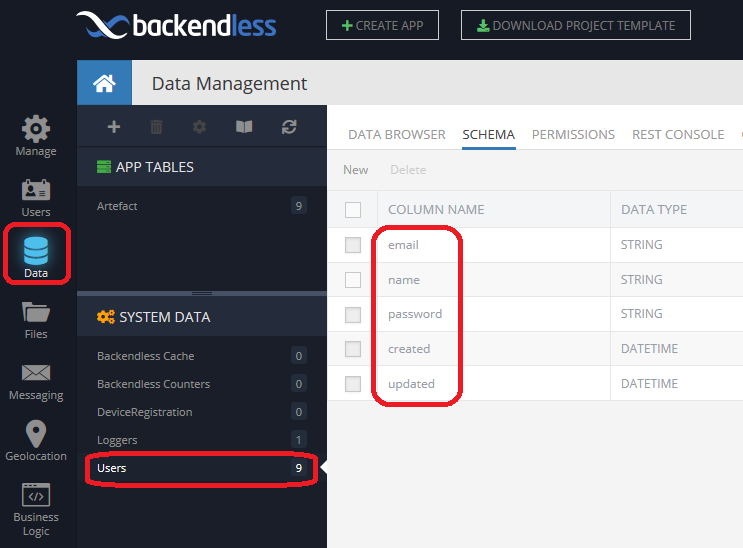
\includegraphics[width=0.8\textwidth]{backendless_console_user_table.png}
	\caption[backendlessConsoleUserTable]{Backendless console user table}
	\label{fig:backendlessConsoleUserTable}
\end{figure}
\footnotetext{URL: https://www.banksy.org [cited 22 August 2018]}


ich realisiere!
														
%---------------------------------------------------------------------------------------------------	
% Der fuenfter Teil der Arbeit
%---------------------------------------------------------------------------------------------------
	%---------------------------------------------------------------------------------------------------
% Tests
%---------------------------------------------------------------------------------------------------
\newpage
%\part{Anfang}
\chapter{Tests}\label{cap:Tests}
ich Teste
														
%---------------------------------------------------------------------------------------------------	
% Der sechster Teil der Arbeit
%---------------------------------------------------------------------------------------------------
	%---------------------------------------------------------------------------------------------------
% Conclusion
%---------------------------------------------------------------------------------------------------
\newpage
%\part{Anfang}
\chapter{Conclusion}\label{cap:Conclusion}

\section{Achievement}
This study was dedicated to the phases of software development for the Civitas project. Doing the analysis, design, realization and test phase, end up in the conclusion. The decision of recreating the app from scratch has made the biggest impact into the process. So it is a question for future developer if it was worth it. To sum up, a working Android application with a lot of additional features was achieved. The following table facilitates the comparison between criteria for success and the achieved outcome.

\begin{table}[h]
\centering
\begin{tabular}{|l|c|}
\hline
\textbf{Criteria for success} & \multicolumn{1}{l|}{\textbf{Achievement}} \\ \hline
List overview for artefacts   & x                                         \\ \hline
Improved filter search        & 1/2                                       \\ \hline
Rating system for artefacts   & -                                         \\ \hline
Password reset                & x                                         \\ \hline
Increased usability           & x                                         \\ \hline
Admin control panel           & x                                         \\ \hline
\end{tabular}
\label{tab:comparison}
\caption{Compare criteria for success with achievements}
\end{table}

Inserting a list overview for artefacts heads to another dimension in the filter search. Unfortunately, the parameter for the artefact owner is not implemented yet. Due to its complexity some bugs are known too. The goal is to eliminate these bugs until the colloquium for this bachelorthesis took place.

A major achievement is not listed in this table, because it is no feature. Nevertheless, it is worth mentioning. Replacing the previous \textbf{REST} back-end architecture with the \textbf{BaaS} by Backendless, guarantees an easy entrance to the Civitas project for the next developer. So if anyone will continue this Civitas project in the future, it is easy as plug and play, because it is just an Android Studio project.
Regrettably, the project has experienced regression in some cases too. At the time the development process was finished, the audio description recording feature for artefacts and the possibility to save more than one image for an artefact was not implementend. 

\section{Known Bugs}
However, a few bugs and faults appear in the Civitas app, at the point the development process was terminated in order to create this document. The current developer tries to remove these until the colloquium was hold. Here is a list of currently known bugs and faults:
\begin{itemize}
\item Missing Internet Permission Request
\item Filtering System
\item Location enable/disable
\item Artefact Retrieval
\end{itemize}

\section{Future Tasks}
On the one hand, there is a working Android app with a lot of functions. On the other hand, as always in the software development, the deeper you are in the matter, the more things you notice. Therefore, here are some suggestions for future tasks the next developer can consider.

\begin{itemize}
\item Swipe refresh method to update list of artefacts
\item Report artefact for abuse
\item Audio description recording for artefacts
\item Share
\item Replace radio buttons with check boxes to allow searching with one or more filter parameters
\item Rating system
\item Thumbnail within marker info window
\item Edit user credentials
\item Multiple image related to a single artefact
\item Comment function for artefacts
\item Retrieve artefacts in relation to the device location
\item Push notification for certain events
\end{itemize}

There is a web application acting as an admin control panel too. These parts are connected by Backendless. So, one can think about, how to optimze the crossplay of these parts get the maximum output. 
														
%---------------------------------------------------------------------------------------------------	
% Literaturverzeichnis
%---------------------------------------------------------------------------------------------------		
  \bibliographystyle{IEEEtranN}   % was dinat        		    														% Anpassung an deutsche Zitierweise
                                          														% Alphabetische Sortierung, Abk�rzungen
  \bibliography{literatur/literatur}    %KAY: WAR DRINNEN   														% Literaturverzeichnis
%  \nocite{linux}
\nocite{xmlHtml}
\nocite{json}
\nocite{androidUdemy}
\nocite{javaUdemy}
\nocite{gitlab}
\nocite{javaScript}
\nocite{activity}
\nocite{bestPractice}
\nocite{fragment}
\nocite{Nefzger}
\nocite{Schirmbacher}

			 %KAY: WAR DRINNEN   																		% hier k�nnen alle Schriftst�cke aufgef�hrt werden, die nicht zitiert, aber dennoch nennenswert sind!
  

											

%---------------------------------------------------------------------------------------------------	
% Anh�nge
%---------------------------------------------------------------------------------------------------	
	\appendix  							%KAY: WAR DRINNEN   
	  	\input{chapter/Endpart/Appendix.tex}
% \input{anhang/hilfsmittel/hilfsmittel}															% Anhang A: Hilfsmittel zur Erstellung
																																			% 					dieser Arbeit
%	\input{anhang/quellcode/quellcode}																	% Anhang B: Quellcode

%---------------------------------------------------------------------------------------------------	
% Glossar
%---------------------------------------------------------------------------------------------------	
	\printnomenclature

%---------------------------------------------------------------------------------------------------	
% Stichwortverzeichnis
%---------------------------------------------------------------------------------------------------	
	\printindex
	
%---------------------------------------------------------------------------------------------------	
% Erkl�rung �ber Selbstst�ndigkeit
%---------------------------------------------------------------------------------------------------		
	\asurency	

%--------------------------------------------------------------------------------------------------- 
% Ende des Schriftst�cks
%--------------------------------------------------------------------------------------------------- 
\end{document}
